\section{The Large Hadron Collider (LHC)}
\label{sec:LHC}
The Large Hadron Collider (LHC)\cite{1748-0221-3-08-S08001}\cite{Bruning:782076}\cite{ipac11:lamont} is the largest and most complex machine every build by man. It is a circular proton-proton collider in a tunnel 100 meters below surface at the CERN research center close to Geneva, inheriting the former Large Electron Positron collider (LEP) tunnel with a circumference of 26.7 km. Fig.~\ref{fig:LHC} shows the layout of the LHC and the vaults containing the experiments. \\
\begin{figure}[tbhn]
\begin{center}
%\begin{tabular}{cc}
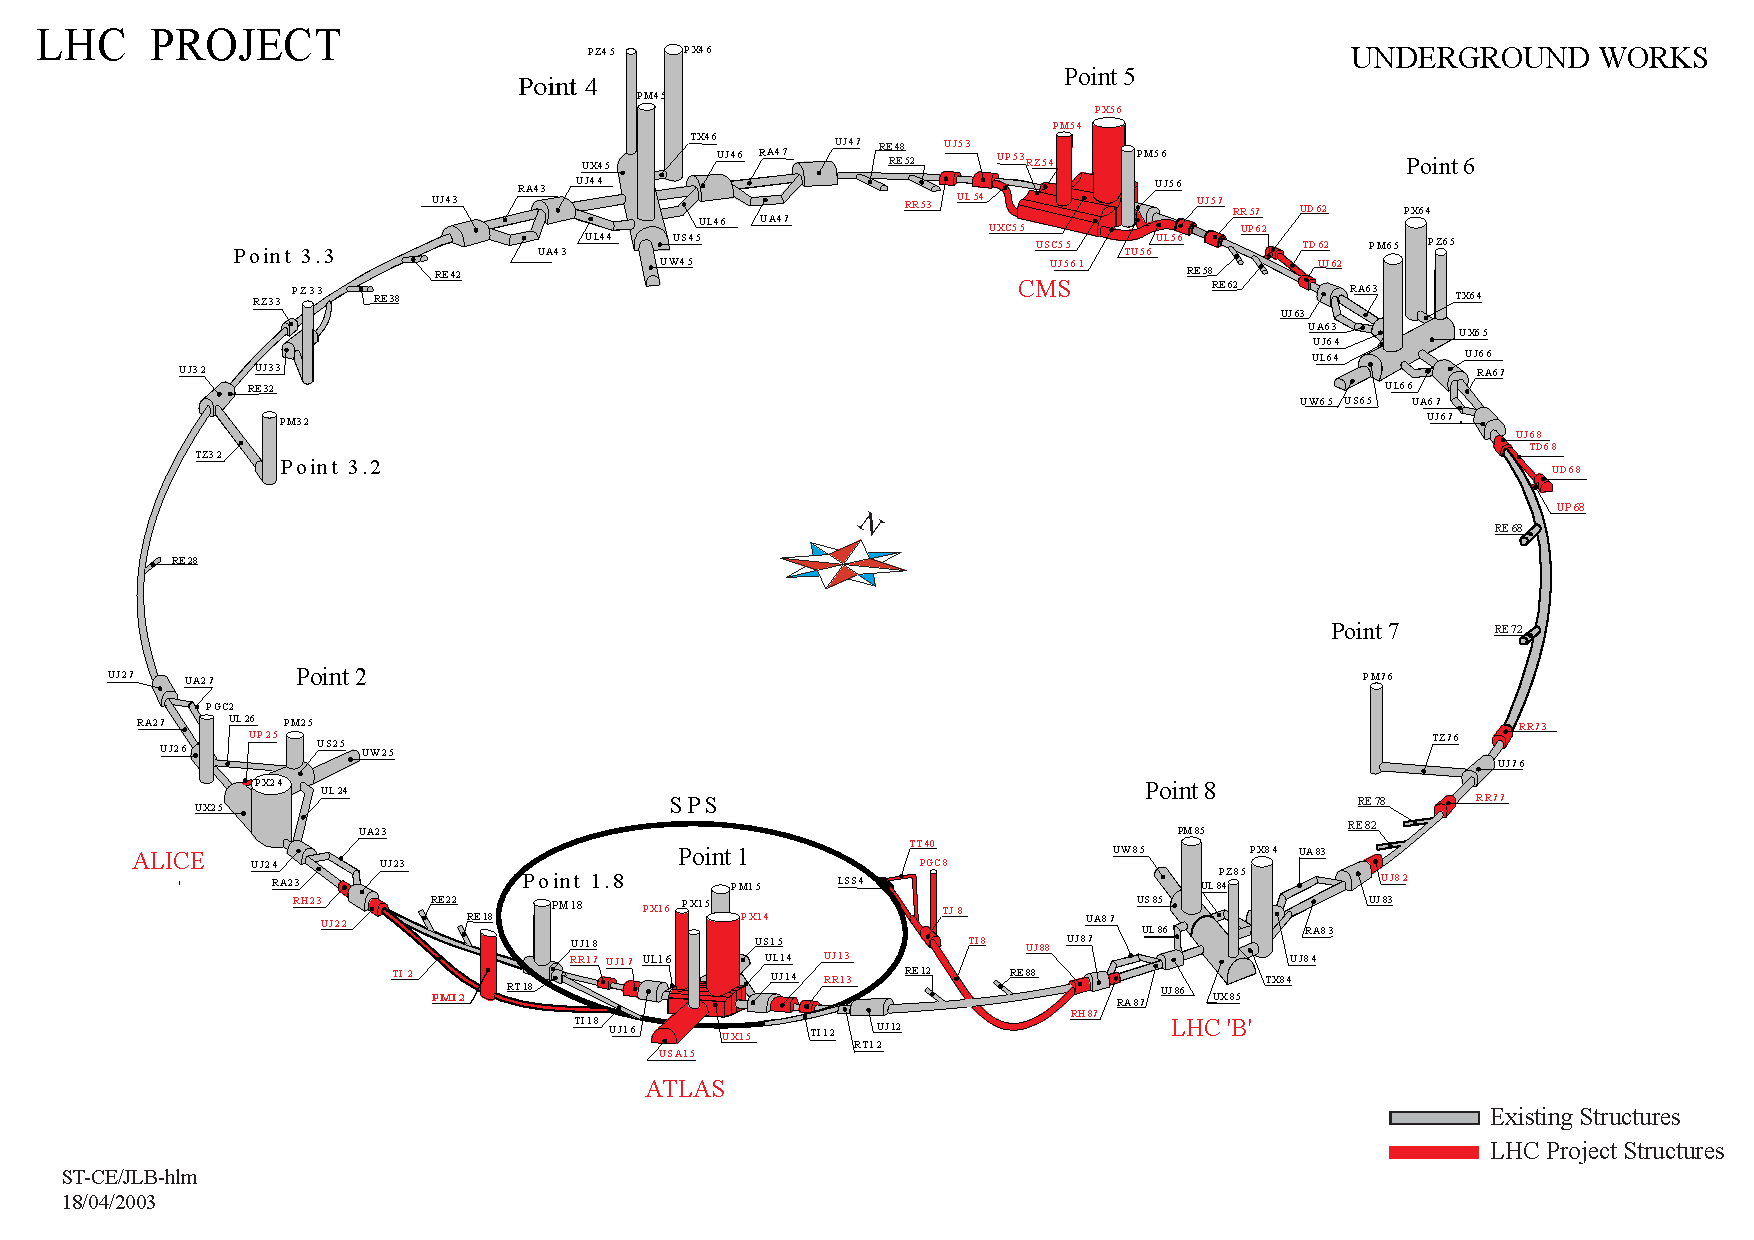
\includegraphics[width=0.85\textwidth]{detector/figures/LHCUnder.pdf}
%\end{tabular}
\end{center}
\caption{An exploded view of the CMS detector.}
%%The bin-by-bin combination of the background contributions and their uncertainties has been performed in a simplified way assuming Gaussian probability distributions.}
\label{fig:LHC}
\end{figure}




The LHC was designed for a center-of-mass energy of 14 TeV and a luminosity of $L = 10^{34} cm^{-2}s^{-1}$. The luminosity $L$ is defined as:
\begin{equation}
 L = \frac{N^{2}_{b}n_{b}f_{rev}\gamma}{4\pi \epsilon_{n}\beta^*}F
\end{equation}
where $N_{b}$ is the number of particles per bunch, $n_b$ the number of bunches per beam, $f_{rev}$ the  revolution frequency, $\gamma$ is the Lorentz factor, $F$ a reduction factor arising from the angel of the two beams at the interaction, $\epsilon_n$ a quantity of the parallelism of the beam and $\beta^*$ is related to the width of the beam at the interaction point.\\
The design Luminosity can be achieved with 2808 bunches colliding every 25 ns, an $\epsilon_n=3.75$ $\mu\text{m}$ and a $\beta^* = 0.55$ m.\\ 
Strong magnetic fields of up to 8,4 Tesla are needed to keep the high energetic protons with a maximum energy of 7 TeV circling. To achieve such high magnetic fields superconducting magnets have been chosen.\\
The particles are collided at specific interaction points at the four main detectors ATLAS\cite{det::ATLAS}, CMS\cite{bib:cmsptdr1}, LHCb\cite{det::LHCb} and ALICE\cite{det::ALICE}.
ATLAS and CMS are multipurpose detector designed with the focus on the discovery of the Higgs boson, search for physics beyond the SM and top physics, while LHCb focuses on the CP-violation in b-physics and ALICEs was designed to investigate quark-gluon plasma produced in heavy ion collisions.\\
This thesis analysis makes use of a total luminosity of \lumi\cite{CMS-PAS-EWK-11-001__} of proton-proton collisions with at a center-of-mass energy of 7 TeV and a peak luminosity of $L = 3.55 \cdot 10^{33} cm^{-2}s^{-1}$ recorded by the CMS detector during the year 2011.\\
The following chapter contains a description of the CMS detector and its components followed by an introduction to the physics objects and definitions relevant for this analyses and the particle flow algorithm used for particle reconstruction.
\clearpage









\section{The Compact Muon Solenoid detector}
One main aspect relevant for the design of the Compact Muon Solenoid (CMS) was the inclusion of the calorimeters within a strong magnetic field to measure charged particles and especially muon momenta to a high precision. To achieve high the magnetic field, a superconducting magnet was installed.\\
The CMS detector is built in cylindrical shape around the beam pipe with a length of 21.6 m and a diameter of 14.6 m with a total weight of of 12 500 tons. Fig.~\ref{fig:CMS} shows an overview of the CMS detector.\\
\begin{figure}[tbhn]
\begin{center}
%\begin{tabular}{cc}
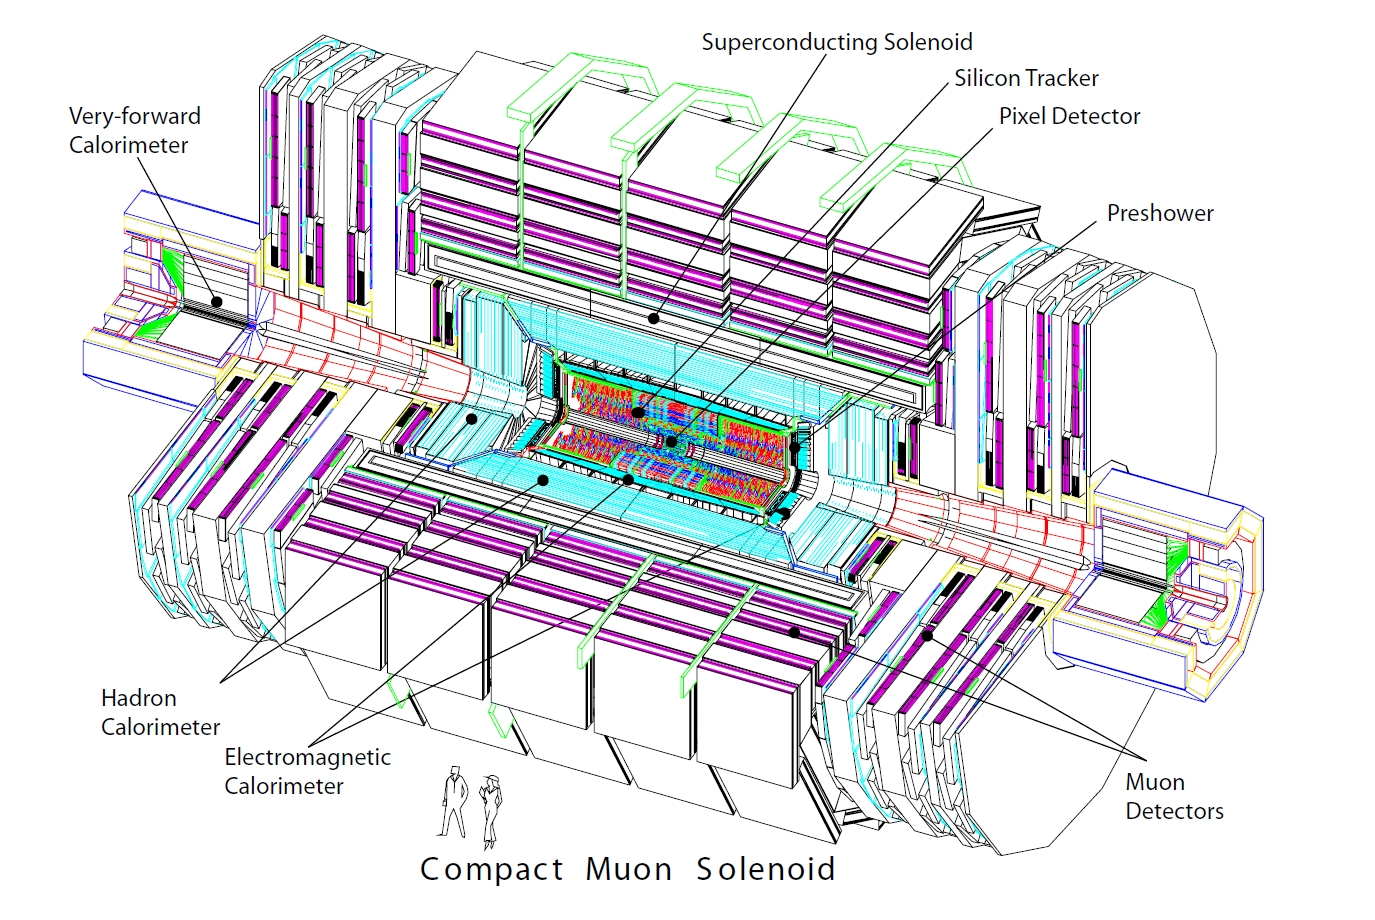
\includegraphics[width=0.85\textwidth]{detector/figures/CMS.jpg}
%\end{tabular}
\end{center}
\caption{An exploded view of the CMS detector.}
%%The bin-by-bin combination of the background contributions and their uncertainties has been performed in a simplified way assuming Gaussian probability distributions.}
\label{fig:CMS}
\end{figure}
\clearpage
A right-handed coordinate system together with cylinder coordinates has been chosen by the CMS collaboration.
With the z-axis pointing in the beam direction, y-axis pointing up and the x-axis pointing to the center of the LHC. The polar angel $\Theta$ is measured from the z-axis and the azimuthal angel $\phi$ is measured relative to the x-axis in the x-y plane.
The pseudorapidity $\eta$, commonly used in high energy physics, is given by:
$$ \eta = - \text{ln tan}\left(\frac{\Theta}{2}\right)  $$
The Lorentz-invariant distance between two relativistic objects is defined as:
$$ \Delta R= \sqrt{(\Delta\eta)^2+(\Delta\Theta)^2} $$
Since the initial momentum in the beam direction (z) for interactions at hadron colliders like the LHC is unknown, only the transverse\footnote{relative to the beam axis} momentum $p_T =p \cdot \text{sin}\Theta$ and the transverse energy $E_T = E \cdot \text{sin}\Theta$ is used to measure the energy and momentum of produced particles.\\
The following layers are cylindrically build around the beam pipe:
\begin{itemize}
 \item A silicon-based tracker (Sec.~\ref{sec:tracker}) at the heart of the detector designed to measure the trajectory of particles with a high precision.
 \item The next layer consists of the electromagnetic calorimeter (ECAL)(Sec.~\ref{sec:ecal}) based on scintillating crystals mainly used to detect electrons and photons.
 \item A preshower system has been installed in front of the ECAL endcaps, designed to identify $\pi^0$ particles.
 \item The Hadronic calorimeter (HCAL)(Sec.~\ref{sec:hcal}) surrounding the electromagnetic calorimeter is designed to measure jet energies.
 \item To improve the HCAL ability to measure high energetic jets a ''tail-catcher'' in the barrel region has also been installed.
 \item The outermost part of the detector consists of the iron yokes for the magnetic field together with the drift chambers together forming the muon detection system (Sec.~\ref{sec:muonchambers}).
\end{itemize}
These sub parts of the CMS detector will be discussed in greater detail in the following.
\clearpage


\subsection{The tracker}
\label{sec:tracker}
Fig. ~\ref{fig:tracker} shows the layout of the CMS tracker\cite{Chatrchyan:2008zzk}\cite{bib:cmsptdr1}\cite{bib:cmstdr:tracker} which extents to 1.1 m in transverse direction and is approximately 5.4 m long.\\
\begin{figure}[tbhn]
\begin{center}
%\begin{tabular}{cc}
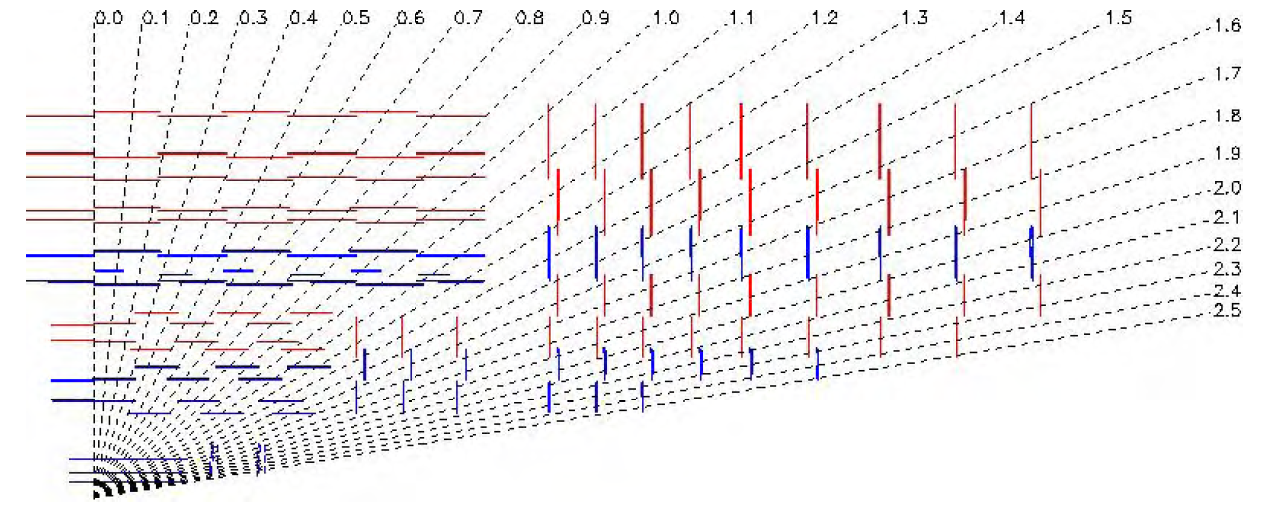
\includegraphics[width=0.85\textwidth]{detector/figures/tracker.png}
%\end{tabular}
\end{center}
\caption{An exploded view of the CMS detector.}
%%The bin-by-bin combination of the background contributions and their uncertainties has been performed in a simplified way assuming Gaussian probability distributions.}
\label{fig:tracker}
\end{figure}
The inner tracker is divided in two parts:\\
The pixel detector consists of 55 million pixels because close to the interaction point a high granularity is necessary due of the high particle flux. Also a high resolution of the vertex reconstruction of 25 $\mu$m and 20 $\mu$ m in X and Y is needed\cite{CMS-PAS-TRK-10-005}. This high resolution is especially important in measurements of b-jets since they have a relative long lifetime resulting in a measurable transverse distance of a second vertex of the decaying b-jet. The high design instantaneous luminosity leads to additional interactions in one bunch-crossing called pileup interactions. These usually soft interactions need to be separated from the hard process which requires good resolution.\\
The second part is the silicon strip detector located outside of the pixel detector. A total area of 200 $\text{m}^2$ is covered by 9.6 million strips covering, the region up to $|\eta| \approx 2.4$.\\
The reconstruction efficiency of muons with a $\pt > 1$ GeV is about 99\%.
Combined with the strong magnetic field tracks of charged particles can be measured to reconstruct the transverse momentum according to this equation:
$$ \pt = 0.3\frac{\text{GeV}}{e \cdot \text{T} \cdot m} \cdot B \cdot \rho$$
with B being the magnetic flux density, $\rho$ the tracks radius of curvature in the transverse plane, $m$ and $e$ being the mass and the electric-charge of the particle.


\subsection{The Electromagnetic Calorimeter}
\label{sec:ecal}
The homogeneous electromagnetic calorimeter (ECAL)\cite{Chatrchyan:2008zzk}\cite{bib:cmsptdr1}\cite{bib:cmstdr:ecal} was build around the inner tracker system consisting of lead-tungstate crystals, which have a radiation length\footnote{The length after which an electrons energy has decreased to $\frac{1}{e}$ of its original energy.} $X_0 = 0.98$ cm and a Moliere radius of $R_M = 2.2$ cm resulting in a compact size which is especially important to fit the tracker, ECAL and the HCAL inside of the Superconducting Solenoid.\\
The barrel part of the ECAL consists of 61 200 crystals covering $|\eta| < 1.479$ whereas the two endcaps are build up of 14 648 crystals covering $ 1.479< |\eta| <3.0$.\\
The crystals are robust against radiation and emit 80\% of the light radiated within the 25 ns between two bunch crossings at design LHC operation. The ECAL has an energy resolution of 
$$ \left(\frac{\sigma}{E} \right)^2= \left(\frac{\text{S}}{\sqrt{E}} \right)^2 +\left(\frac{\text{N}}{E}\right)^2+ \text{C}^2 $$
with S=3\% as stochastic term, N = 124 MeV as noise term and C = 0.26\% as constant term.	
The response of a calorimeter is defined to be the measured energy divided by the true energy of a particle showering. Hadrons and electrons have a different response with the ratio given by $\frac{e}{h}\approx 1.6$. Noise is being suppressed by only reading out cells with an energy deposited above a certain threshold.\\
Good performance of the ECAL has been observed however some of the about 70 000 crystals have a dysfunctional readout.


\subsection{The Hadronic Calorimeter}
\label{sec:hcal}
The Hadronic Calorimeter (HCAL)\cite{Chatrchyan:2008zzk}\cite{bib:cmsptdr1}\cite{bib:cmstdr:hcal} consists of alternating layers of brass as absorber and plastic scintillators. To support these heavy structures the innermost and outermost layers are made of steel. The ECAL and HCAL are arranged in towers read out by single wavelength shifting fibers.\\
The HCAL consists of four parts:
\begin{itemize}
 \item The hadron barrel (HB) covering the central part of the HCAL with $|\eta| < 1.4$ made of 2304 towers with a segmentation of $\Delta \eta$ x $\Delta \Phi = 0.087$ x $0.087$. The absorbers have the thickness of 5.05 cm for each of the inner eight layers and 5.56 for the outer six layers. The scintillators located in between the absorber layers are 3.7 mm thick except for the very first layer behind the ECAL which is 9 mm thick. 
 \item Due to the limited space available by keeping the HCAL inside the Solenoid, jets may not deposit their entire energy within this part. Scintillators are also outside the coil with an interaction length of 1.4/sin($\Theta$) called the hadron outer detector (HO)\footnote{This part was not used for the analyzed data in this thesis since the noise level was not sufficiently small.}.
 \item The hadron endcaps (HE) make up the third part. Here only 87 mm thick brass and one 3.7 mm thick scintillator was used. 
 \item The last part the hadron forward (HF) is located close to the beam axis at   $3.0 <|\eta| < 5.0$. This part is made of steel absorber and radiation hard quartz fibers. It is constructed out of 18 wedges located 11 m from the interaction point thus increasing the coverage helping to measure missing transverse momentum.
\end{itemize}
Like the ECAL the HCAL is a non-compensating calorimeter with $\frac{\text{e}}{\text{h}}\approx 1.4$. A read out threshold is also used to reduce noise (called zero suppression).



\clearpage
\subsection{The Solenoid and the Muon Chambers}
\label{sec:muonchambers}
The superconducting solenoid with a length of 12.9 m, a thickness of 1.8 m and an inner diameter of 5.9 m is one of key element of the CMS detector dominating its design. 19.5 kA of current are used to provide the 3.8 Tesla magnetic field which permeates the calorimeter and tracker.\\
The muon chambers\cite{Chatrchyan:2008zzk}\cite{bib:cmsptdr1}\cite{bib:cmstdr:muon} localed outside the magnetic coil partially taking advantage of the material used for the solenoid consist of four muon stations covering $|\eta|<2.4$.
The muon barrel region (MB) uses aluminum drift tube chambers (DT) to achieve high resolution for muons. The endcaps (ME) consist of cathode strip chambers (CSCs). In this forward direction a higher rate of muons is expected explaining the use of CSCs due to their fast response. The coverage is being completed by resistive plate chambers (RPCs) included in both parts of the muon chambers. These RPCs have a much lower momentum resolution than the other parts of the muon chambers but the very fast response time and the excellent time resolution is needed to identify the correct bunch crossing. These muon detectors are arranged in four stations in both detector regions.\\
Together with the inner tracker the muon system is able to achieve a muon \pt resolution between 1\% and 10\% up to a muon \pt of 1 TeV.




\subsection{Trigger}
\label{sec:trigger}
At design luminosity the LHC has a bunch crossing rate of 40 MHz. At this rate the event size of approximately  1 MB per event leads to a too high output of data to be stored and processed. Since not all events include interesting physics a trigger system\cite{bib:cmstdr:trigger}\cite{bib:trigger:summerschoollecture} only collecting events fulfilling predefined criteria is installed.\\
The trigger is organized in two stages:
\begin{itemize}
 \item The pure hardware\footnote{Pure hardware trigger was chosen since it has increased speed compared to software triggers.} level 1 trigger(L1) using only detector parts which have a fast readout rate, the calorimeters and the muon chambers. These informations are combined by simplified object algorithms to loosely define electrons, photons, muons and jets. From these algorithms interesting events are selected by demanding a certain energy threshold and or leptons or jets to reduce the event rate to 100 kHz\footnote{Prescaled trigger paths are used to collect only every x-th collision of one type of interaction, important for collisions which have a too high rate to recored every collision.}. To keep the information until the L1 has decided weather an event will rejected or not the full detector output is stored in a pipeline for 3.2 $\mu$s.
 \item The software based high level trigger (HLT) which is also used to reduce the amount of events further by a factor of 100 to be able to store the events at a rate of $\approx 100$ MB/s. This trigger can access the full detector information enabling more advanced trigger algorithm definitions. The advantage of software based triggers compared to hardware based ones is the flexibility in the design of individual trigger paths. Restrictions from the aim of a reduction factor of 100 together with the demands from physical analysis dominate the trigger paths designs. 
\end{itemize}
Each stored event inherits the L1 and HLT trigger informations.
 

\section{Particle identification and physical object definitions}
\label{sec:physics_objects}
This section covers particle identification of the CMS detector and physics quantities used in this thesis.\\
The particles emerging from the interaction point at the center interact differently with the detector components enabling distinguishing between them. Fig.~\ref{fig:particlePassing} illustrates typical interactions with the detector components.
\begin{figure}[tbhn]
\begin{center}
%\begin{tabular}{cc}
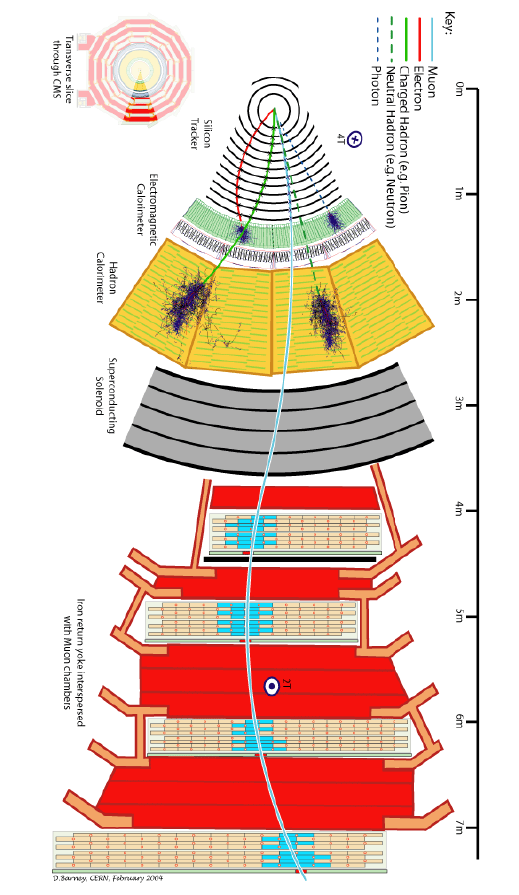
\includegraphics[width=0.75\textwidth]{detector/figures/particlePassing.png}
%\end{tabular}
\end{center}
\caption{This figure shows the transverse slice through the CMS detector with typical particle interaction signatures with the detector.}
%%The bin-by-bin combination of the background contributions and their uncertainties has been performed in a simplified way assuming Gaussian probability distributions.}
\label{fig:particlePassing}
\end{figure}

This list covers typical signatures of photons, electrons, muons, taus, jets and only weakly interacting particles:

\begin{itemize}
 \item Photons are electrical neutral particles thus leaving in most cases no track in the tracker. First interactions happens typically in the ECAL. Due to the depth of $X_0=25$ of the ECAL photons are most likely to deposit all energy distributed only over a few crystals in the ECAL. Approximately 50\% of all photons already convert to $e^-e^+$ pairs within the tracker but usually the major fraction of energy is deposited in the ECAL\cite{CMS-PAS-EGM-10-005}.
 \item Electron identification is difficult because of the emission of Bremsstrahlung. Due to the high magnetic field and the strong resulting bending of the electron trajectory the emitted photons are spread across the detector. Clustering algorithms are used to take Bremsstrahlung into account. In particular Superclusters (clusters of clusters) together with a matched track from the tracker are used in the reconstruction of electrons\cite{CMS-PAS-EGM-10-004}.  
 \item Muons with a $p_t> 2.5$ GeV loose only a small fraction of their energy within the detector\cite{CMS-PAS-MUO-10-002} making them so so called minimize ionizing particles. They are the only particles that reach the muon chambers making the muon identification very easy.
 \item Taus have a too short lifetime to interact with the detector. Instead only the decay products can be observed. Their are  special algorithms designed to identify taus but this thesis does not include any tau signatures.
 \item In the hard interaction\footnote{Hard interactions refer to a high energy transfer in the parton parton interaction.} quarks and gluons may be produced. As discussed in Sec.~\ref{sec:qcd} color charged particles can only exist in bound states leading to the formation of jets which consist of many emitted hadrons close to each other. These hadrons can either be electrically neutral, leaving no track in the tracking system or electrically charged. Neutral hadrons will only interact with the HCAL whereas charged hadrons also leave a signal in the tracker and the ECAL. The main fraction of energy of both types is always deposited within the HCAL. The effect referred to as ''punch through'' occurs when a jet has too much energy to be stopped within the HCAL. This is the main source for high energetic jet mismeasurements. 
 \item Weakly interacting particles will not interact with any component of the detector. They can only be measured indirectly by taking advantage of the initial state of no transverse momentum. An imbalance in the transverse momentum plane hints to the production of, such a particle. 
\end{itemize}

These particles are all reconstructed with the particle flow algorithm discussed in  Sec.~\ref{sec:particleflow}. The reconstructed particles are used for the following physical quantities:
\begin{itemize}
 \item $\HT=\sum|\vec{\pt}|$, only jets with $|\vec{\pt}| > 50 \xspace$ GeV and$|\eta| < 2.5$ are considered.
 \item $\MHT = -\sum (\vec{\pt})$, jets with $|\vec{p_{T}}| > 30$ GeV and $|\eta| < 5$ are included. A different selection than for \HT is used to avoid introducing artificial \MHT by neglecting jets.
 \item $\met = -\sum (\vec{\pt})$, all particles \pt found in an event.
\end{itemize}


\section{The particle-flow algorithm}
\label{sec:particleflow}

The particle-flow algorithm used by CMS is based on the idea to reconstruct all stable particles. An important ingredient is the combination of all detector component information in the particle reconstruction procedure. 
The first step is the definition of elementary signatures. One being the identification of charged particles from inner tracker and muon chamber informations. Another is the clustering procedure. Calorimeter information is used to define clusters from adjacent calorimeter cells with energy deposits.\\ 
Since particles can have several of these signatures they are linked to blocks in order to improve accuracy by combining signatures from different subdetector parts and to avoid double-counting of signatures. For example Bremsstrahlung photons  are tried to be identify by matching tangential extrapolated clusters from the ECAL to a track in the tracker. The resolution of muons is improved by linking tracks from the inner tracker with the muon system.\\
The final particle reconstruction is done according to dedicated quality criteria. For each identified particle the tracks and energy deposition are removed from an event to avoid double counting.\\
First the muons are identified, followed by the electrons. The remaining tracks are considered to be charged hadrons tracks and are matched to clusters energies. HCAL and ECAL clusters that can not be matched to a track are interpreted as neutral hadrons. Photons are identified if only ECAL clusters remain that can not be matched to a track.\\
The particle-flow algorithm has improved especially the jet measurements performance\cite{CMS-PAS-PFT-09-001}\cite{1748-0221-6-11-P11002}.
